% \iffalse
\let\negmedspace\undefined
\let\negthickspace\undefined
\documentclass[journal,12pt,twocolumn]{IEEEtran}
\usepackage{cite}
\usepackage{amsmath,amssymb,amsfonts,amsthm}
\usepackage{algorithmic}
\usepackage{graphicx}
\usepackage{textcomp}
\usepackage{xcolor}
\usepackage{txfonts}
\usepackage{listings}
\usepackage{enumitem}
\usepackage{mathtools}
\usepackage{gensymb}
\usepackage{comment}
\usepackage[breaklinks=true]{hyperref}
\usepackage{tkz-euclide} 
\usepackage{listings}
\usepackage{gvv}                                        
\def\inputGnumericTable{}                                 
\usepackage[latin1]{inputenc}                               \usepackage{caption}
\usepackage{color}                                            
\usepackage{array}                                            
\usepackage{longtable}                                       
\usepackage{calc}                                             
\usepackage{multirow}                                         
\usepackage{hhline}                                           
\usepackage{ifthen}                                           
\usepackage{lscape}

\newtheorem{theorem}{Theorem}[section]
\newtheorem{problem}{Problem}
\newtheorem{proposition}{Proposition}[section]
\newtheorem{lemma}{Lemma}[section]
\newtheorem{corollary}[theorem]{Corollary}
\newtheorem{example}{Example}[section]
\newtheorem{definition}[problem]{Definition}
\newcommand{\BEQA}{\begin{eqnarray}}
\newcommand{\EEQA}{\end{eqnarray}}
\newcommand{\define}{\stackrel{\triangle}{=}}
\theoremstyle{remark}
\newtheorem{rem}{Remark}
\begin{document}

\bibliographystyle{IEEEtran}
\vspace{3cm}

\title{Audio filtering}
\author{EE23BTECH11010 - Venkatesh Bandawar$^{*}$% <-this % stops a space
}
\maketitle
\newpage
\bigskip

\renewcommand{\thefigure}{\arabic{figure}}
\renewcommand{\thetable}{\arabic{table}}

\bibliographystyle{IEEEtran}

\begin{table}[htbp] 
\centering
\begin{tabular}{|c|c|}
\hline
\textbf{Parameter} & \textbf{Description}\\
     \hline
     x(n) & Input Audio Signal \\
     \hline
     y(n) & Output Audio Signal\\ 
     \hline
     H(z) & Discrete Time Fourier Transform of x(n)\\
     \hline
     h(n) & Impulse Response\\
     \hline
\end{tabular}

\caption{Input Table}
\end{table}

Frequency Response of Input Audio signal $x\brak{n}$, given as :
\begin{figure}[!h] 
\centering
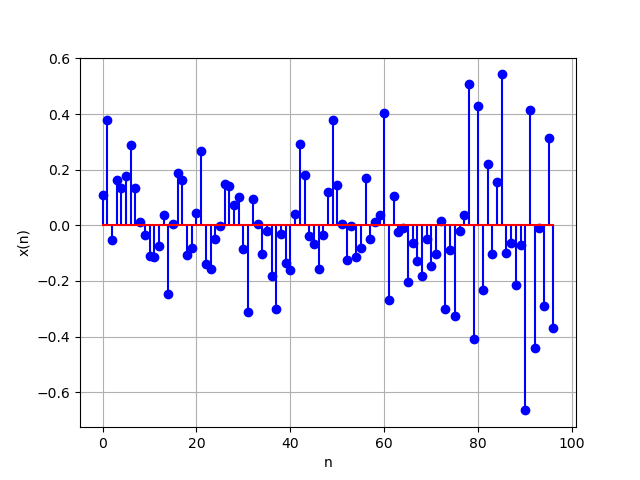
\includegraphics[width=\columnwidth]{figs/x(n).png}
\caption{Graph of x(n)}
\end{figure}

The Output response can be obtained from Difference equation, given as :\\
\begin{align}
    \sum _{m=0}^{M}a\brak{m}y\brak{n-m}=\sum _{k=0}^{N}b\brak{k}x\brak{n-k}
\end{align}
The values of $a$ and $b$ are obtained in 'filter.py'  file.

\begin{align}
    x[n] \system{\mathcal{F}} X(\omega)\\
    y[n] \system{\mathcal{F}} Y(\omega)\\
    h[n] \system{\mathcal{F}} H(\omega)
\end{align}

\begin{figure}[!h] 
\centering
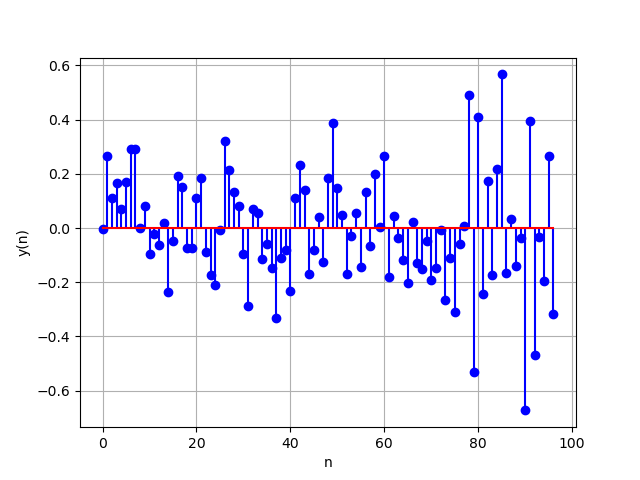
\includegraphics[width=\columnwidth]{figs/y(n).png}
\caption{Graph of y(n)}
\end{figure}
\newpage

The plot of $H(\omega)$ is given as :
\begin{figure}[!h] 
\centering
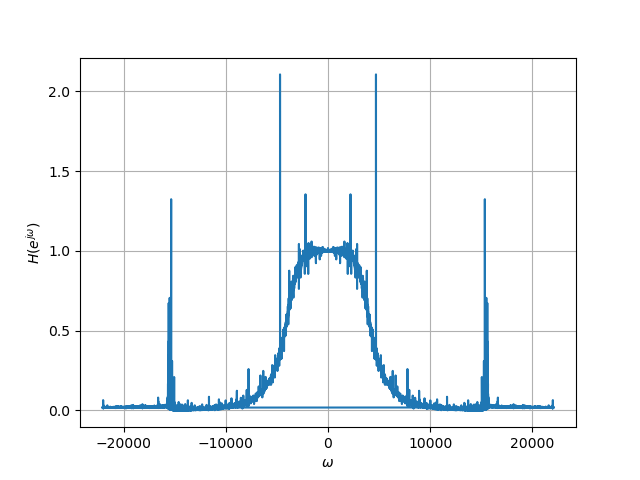
\includegraphics[width=\columnwidth]{figs/H(w).png}
\caption{Graph of $H(\omega)$}
\end{figure}

$H(\omega)$ is taken as : $\dfrac{X(\omega)}{Y(\omega)}$
\begin{align}
    H(\omega) \mathrel{\substack{\mathcal{F}^{-1}\\\longleftrightarrow}} h(n)
\end{align}
Taking Inverse fourier transform of $H(\omega)$
\begin{figure}[!h] 
\centering
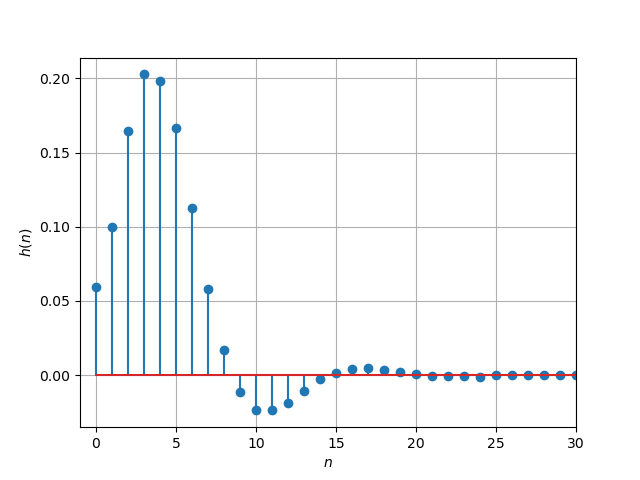
\includegraphics[width=\columnwidth]{figs/h(n).png}
\caption{Graph of h(n)}
\end{figure}

\end{document}
